%% bare_jrnl.tex
%% V1.4b
%% 2015/08/26
%% by Michael Shell
%% see http://www.michaelshell.org/
%% for current contact information.
%%
%% This is a skeleton file demonstrating the use of IEEEtran.cls
%% (requires IEEEtran.cls version 1.8b or later) with an IEEE
%% journal paper.
%%
%% Support sites:
%% http://www.michaelshell.org/tex/ieeetran/
%% http://www.ctan.org/pkg/ieeetran
%% and
%% http://www.ieee.org/

%%*************************************************************************
%% Legal Notice:
%% This code is offered as-is without any warranty either expressed or
%% implied; without even the implied warranty of MERCHANTABILITY or
%% FITNESS FOR A PARTICULAR PURPOSE! 
%% User assumes all risk.
%% In no event shall the IEEE or any contributor to this code be liable for
%% any damages or losses, including, but not limited to, incidental,
%% consequential, or any other damages, resulting from the use or misuse
%% of any information contained here.
%%
%% All comments are the opinions of their respective authors and are not
%% necessarily endorsed by the IEEE.
%%
%% This work is distributed under the LaTeX Project Public License (LPPL)
%% ( http://www.latex-project.org/ ) version 1.3, and may be freely used,
%% distributed and modified. A copy of the LPPL, version 1.3, is included
%% in the base LaTeX documentation of all distributions of LaTeX released
%% 2003/12/01 or later.
%% Retain all contribution notices and credits.
%% ** Modified files should be clearly indicated as such, including  **
%% ** renaming them and changing author support contact information. **
%%*************************************************************************


% *** Authors should verify (and, if needed, correct) their LaTeX system  ***
% *** with the testflow diagnostic prior to trusting their LaTeX platform ***
% *** with production work. The IEEE's font choices and paper sizes can   ***
% *** trigger bugs that do not appear when using other class files.       ***                        
% The testflow support page is at:
% http://www.michaelshell.org/tex/testflow/



\documentclass[journal]{IEEEtran}
%
% *** GRAPHICS RELATED PACKAGES ***
%
\usepackage{graphicx} 
\ifCLASSINFOpdf
  % \usepackage[pdftex]{graphicx}
  % declare the path(s) where your graphic files are
  % \graphicspath{{../pdf/}{../jpeg/}}
  % and their extensions so you won't have to specify these with
  % every instance of \includegraphics
  % \DeclareGraphicsExtensions{.pdf,.jpeg,.png}
\else
  % or other class option (dvipsone, dvipdf, if not using dvips). graphicx
  % will default to the driver specified in the system graphics.cfg if no
  % driver is specified.
  % \usepackage[dvips]{graphicx}
  % declare the path(s) where your graphic files are
  % \graphicspath{{../eps/}}
  % and their extensions so you won't have to specify these with
  % every instance of \includegraphics
  % \DeclareGraphicsExtensions{.eps}
\fi
% graphicx was written by David Carlisle and Sebastian Rahtz. It is
% required if you want graphics, photos, etc. graphicx.sty is already
% installed on most LaTeX systems. The latest version and documentation
% can be obtained at: 
% http://www.ctan.org/pkg/graphicx
% Another good source of documentation is "Using Imported Graphics in
% LaTeX2e" by Keith Reckdahl which can be found at:
% http://www.ctan.org/pkg/epslatex
%
% latex, and pdflatex in dvi mode, support graphics in encapsulated
% postscript (.eps) format. pdflatex in pdf mode supports graphics
% in .pdf, .jpeg, .png and .mps (metapost) formats. Users should ensure
% that all non-photo figures use a vector format (.eps, .pdf, .mps) and
% not a bitmapped formats (.jpeg, .png). The IEEE frowns on bitmapped formats
% which can result in "jaggedy"/blurry rendering of lines and letters as
% well as large increases in file sizes.
%
% You can find documentation about the pdfTeX application at:
% http://www.tug.org/applications/pdftex


% correct bad hyphenation here
\hyphenation{op-tical net-works semi-conduc-tor}


\begin{document}
%
% paper title
% Titles are generally capitalized except for words such as a, an, and, as,
% at, but, by, for, in, nor, of, on, or, the, to and up, which are usually
% not capitalized unless they are the first or last word of the title.
% Linebreaks \\ can be used within to get better formatting as desired.
% Do not put math or special symbols in the title.
\title{Improving Sign Recognition Models with Blender-Synthesized Data}
%
%
% author names and IEEE memberships
% note positions of commas and nonbreaking spaces ( ~ ) LaTeX will not break
% a structure at a ~ so this keeps an author's name from being broken across
% two lines.
% use \thanks{} to gain access to the first footnote area
% a separate \thanks must be used for each paragraph as LaTeX2e's \thanks
% was not built to handle multiple paragraphs
%

% Names listed in alphabetical order of first name. 
\author{
    Deekshith Dade\textsuperscript{1},
    Hunter Rogers\textsuperscript{1},
    Mihir Rane\textsuperscript{1},
    William J. Anderl\textsuperscript{1},
    Yi-Kai Lee\textsuperscript{1},
    David Sacharny\textsuperscript{2},
    Thomas~C.~Henderson\textsuperscript{1}
    \thanks{1: University of Utah, Salt Lake City, Utah, email: \tt\small tch@cs.utah.edu}
    \thanks{2: Add david's info, email: }
}



% note the % following the last \IEEEmembership and also \thanks - 
% these prevent an unwanted space from occurring between the last author name
% and the end of the author line. i.e., if you had this:
% 
% \author{....lastname \thanks{...} \thanks{...} }
%                     ^------------^------------^----Do not want these spaces!
%
% a space would be appended to the last name and could cause every name on that
% line to be shifted left slightly. This is one of those "LaTeX things". For
% instance, "\textbf{A} \textbf{B}" will typeset as "A B" not "AB". To get
% "AB" then you have to do: "\textbf{A}\textbf{B}"
% \thanks is no different in this regard, so shield the last } of each \thanks
% that ends a line with a % and do not let a space in before the next \thanks.
% Spaces after \IEEEmembership other than the last one are OK (and needed) as
% you are supposed to have spaces between the names. For what it is worth,
% this is a minor point as most people would not even notice if the said evil
% space somehow managed to creep in.



% The paper headers
% \markboth{Journal of \LaTeX\ Class Files,~Vol.~14, No.~8, August~2015}%
% {Shell \MakeLowercase{\textit{et al.}}: Bare Demo of IEEEtran.cls for IEEE Journals}
% The only time the second header will appear is for the odd numbered pages
% after the title page when using the twoside option.
% 
% *** Note that you probably will NOT want to include the author's ***
% *** name in the headers of peer review papers.                   ***
% You can use \ifCLASSOPTIONpeerreview for conditional compilation here if
% you desire.




% If you want to put a publisher's ID mark on the page you can do it like
% this:
%\IEEEpubid{0000--0000/00\$00.00~\copyright~2015 IEEE}
% Remember, if you use this you must call \IEEEpubidadjcol in the second
% column for its text to clear the IEEEpubid mark.



% use for special paper notices
%\IEEEspecialpapernotice{(Invited Paper)}




% make the title area
\maketitle

% As a general rule, do not put math, special symbols or citations
% in the abstract or keywords.
\begin{abstract}
Road-sign condition and content is critically important globally for drivers safety and critical infrastructure maintenence. Several groups have developed methods to detect and evaluate various sign metrics. Additionally, growing interest in autonomous driving requires input from road-signs for critical decision making. Data acquisition and cleaning is an ongoing challenge when training deep learning models, and is commonly a limiting factor of model performance. In sign recognition, this problem is exacerbated by the many different variations in typical signage between geographic locations. Here, we establish the validity of using synthetic data, generated using Blender, to improve sign detection and discuss the advantages of using synthetically generated datatsets for deep learning tasks.    
\end{abstract}

% Note that keywords are not normally used for peerreview papers.
% \begin{IEEEkeywords}
% IEEE, IEEEtran, journal, \LaTeX, paper, template.
% \end{IEEEkeywords}






% For peer review papers, you can put extra information on the cover
% page as needed:
% \ifCLASSOPTIONpeerreview
% \begin{center} \bfseries EDICS Category: 3-BBND \end{center}
% \fi
%
% For peerreview papers, this IEEEtran command inserts a page break and
% creates the second title. It will be ignored for other modes.
\IEEEpeerreviewmaketitle



\section{Introduction}
% The very first letter is a 2 line initial drop letter followed
% by the rest of the first word in caps.
% 
% form to use if the first word consists of a single letter:
% \IEEEPARstart{A}{demo} file is ....
% 
% form to use if you need the single drop letter followed by
% normal text (unknown if ever used by the IEEE):
% \IEEEPARstart{A}{}demo file is ....
% 
% Some journals put the first two words in caps:
% \IEEEPARstart{T}{his demo} file is ....
% 
% Here we have the typical use of a "T" for an initial drop letter
% % and "HIS" in caps to complete the first word.
% \IEEEPARstart{T}{his} demo file is intended to serve as a ``starter file''
% for IEEE journal papers produced under \LaTeX\ using
% IEEEtran.cls version 1.8b and later.
% % You must have at least 2 lines in the paragraph with the drop letter
% % (should never be an issue)
% I wish you the best of success.

% \hfill mds
 
% \hfill August 26, 2015
Road signs are an invaluable component of global transportation infrastructure. Signs provide information concerning local transportation laws and regulations such as road speed and required stopping points, as well as tailored instructions for drivers on a specific section of road. As such, signs may be both standardized and vary widely depending on region. Due to the complexity and importance of road signage, the recognition, classification, and interpretation of road signs is applicable to a variety of deep learning goals[Insert citation here]. Data acquisition, cleaning, and labeling is commonly recognized as a major limiting factor when training deep learning models\cite{Whang_datacollection}, with sign data being no exception. Dashboard cameras (dashcams) are commonly used both to collect training data and provide continously up to date images which are then passed to pre-trained models. Dashcam footage has its own inherent drawbacks however including motion artifacts and debris obstruction. Perhaps the most limiting factor, however, is the time and resources required to obtain dashcam footage of the desired sign in a specific location and orientation, as well as labeling the collected images correctly. We hypothesize that artifical data, generated with a free modeling software, can fill the data acquisition gap by providing rapidly produced labeled images featuring custom or pre-built signs in various locations, orientations, and conditions. 

\section{Previous Work}

 Synthetic data generation for sign detection is not an entirely novel approach. Several groups have explored using synthetic data to augment existing training data sets. Villalonga et al. proposed the use of Generative Adversarial Networks (GANs) to rapidly add new sign classes to datasets, which while effective, was limited by the choice of classification and generation models \cite{GAN_artificial_data}. This differs from our approach because XXXXXXXX. Similarly, Soans et al. created a similar Blender approach, in which signs were created with various software and placed on a real image background \cite{blender_paper}. This differs significantly from our proposed approach, in which we create an entirely synthetic scene. There are existing packages that create 3D road scenes, namely CARLA simulator [XXXXX]. However, the process of creating custom sign objects to place into CARLA is generally complicated, and requires users to adjust object mesh directly. While significant efforts have been made to synthesize sign data, improvements to both performance and workflow are needed to optimize dataset comprehensiveness and real-world applicability. 
\section{Methods}
Blender may be controlled without using a user interface via the Blender Python API, which allows for python scripting to replace traditional blender inputs. As the intention of this tool is to allow users to easily integrate data generation into a deep learning pipeline, all scene generation was created using Blender scripting, with the input being a simple JSON file that a user may adjust within certain presets to adjust various scene variables, listed below. Images are output already correctly labeled, and ready to be added to training datasets. 
\subsection{Signs}
Signs were created by collecting a variety of images of common signs in the United States. These signs were then converted to a protable network graphic (PNG) format with a transparent background. In Blender, the sign is applied to a mesh object such that the background of the object is transparent, leaving only the sign in place. This allows for seamless scaling, as well as allowing the user to prepare any PNG as a sign. In order for more realistic images, various damage states and sign orientations may be randomly applied to the sign. Finally, various weather conditions such as snow and mud may be added to the front of the sign, as obstruction due to environmental factors is common in harsher climates. Signs are placed on a simple pole, and positioned correctly within the scene relative to a camera object. 

\begin{figure}[ht]
    \centering
    \begin{minipage}{0.1\textwidth}
        \centering
        
\includegraphics[width=\linewidth]{images/All Way Stop.png}

    \end{minipage}\hfill
    \begin{minipage}{0.1\textwidth}
        \centering
        
\includegraphics[width=\linewidth]{images/Bump.png}

    \end{minipage}\hfill
    \begin{minipage}{0.1\textwidth}
        \centering
        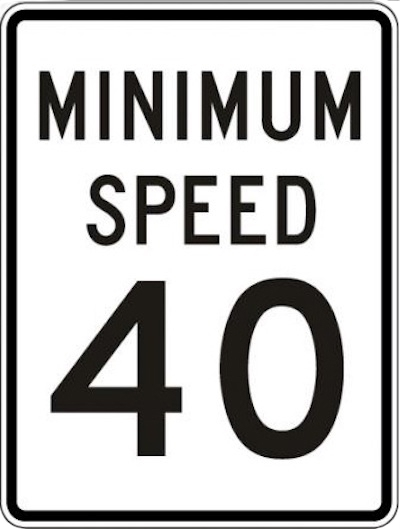
\includegraphics[width=\linewidth]{images/Minimum Speed 40.png}

    \end{minipage}
    \caption{Representative samples of signs input images}
    \label{fig:row_of_images}
\end{figure}

\subsection{Roads}
Preset road scenes were similarly created via Python scripting. A simple two-lane road, as well as a highway scene were constructed using free mesh objects and textures from BlenderKit[XXXX], but could be recreated using a variety of available Blender resources. Roads include concrete barriers, guardrails, lighting, and lane divisions. Optionally, the road was curved in the 3D space, with lane coordinates returned to allow the camera object to move along each lane to correctly imitate real-world roads. 
\subsection{Environment}
Each road was placed on a plane which may be changed between various pre-set images to simulate diverse environments. Similar to the road objects, this plane was randomly curved in the 3D space to match the orientation of the road, effectively simulating topological changes, which affect both camera placement and sign visualization as the camera moves through the simulated scene. Additionally, different weather conditions including snow, rain, and fog were used to expand the dataset to include environmental obstructions of the sign directly within the camera field of view. 

One of the main benefits of using a free platform such as Blender is that there are a wide variety of plugins, both free and paid, which can be used to improve scene creation. Here, a tree add-on was used to generate different styles of trees, which were then randomly scattered in the scene. 

\subsection{Camera and Lighting}
A camera object was placed within the blender scene, which follows the path of each road lane for a user-specified number of steps. An image was placed in the distance, attached to the camera, such that there was always a simulated sky behind the sign. Lighting was also added via Blender's light object, which allowed for simulations of shadows, reflections, and other lighting aberations, a significant improvement from previous Blender image-generation strategies\cite{blender_paper}. 

\subsection{Annotations}
All images were rendered and stored following the Common Objects in Context (COCO) annotation scheme for later ease of use. As the scene variables were carefully controlled, each generated image contains metadata including scene variables as well as a bounding box for the sign within the image. 

\begin{figure}[ht]
    \centering
    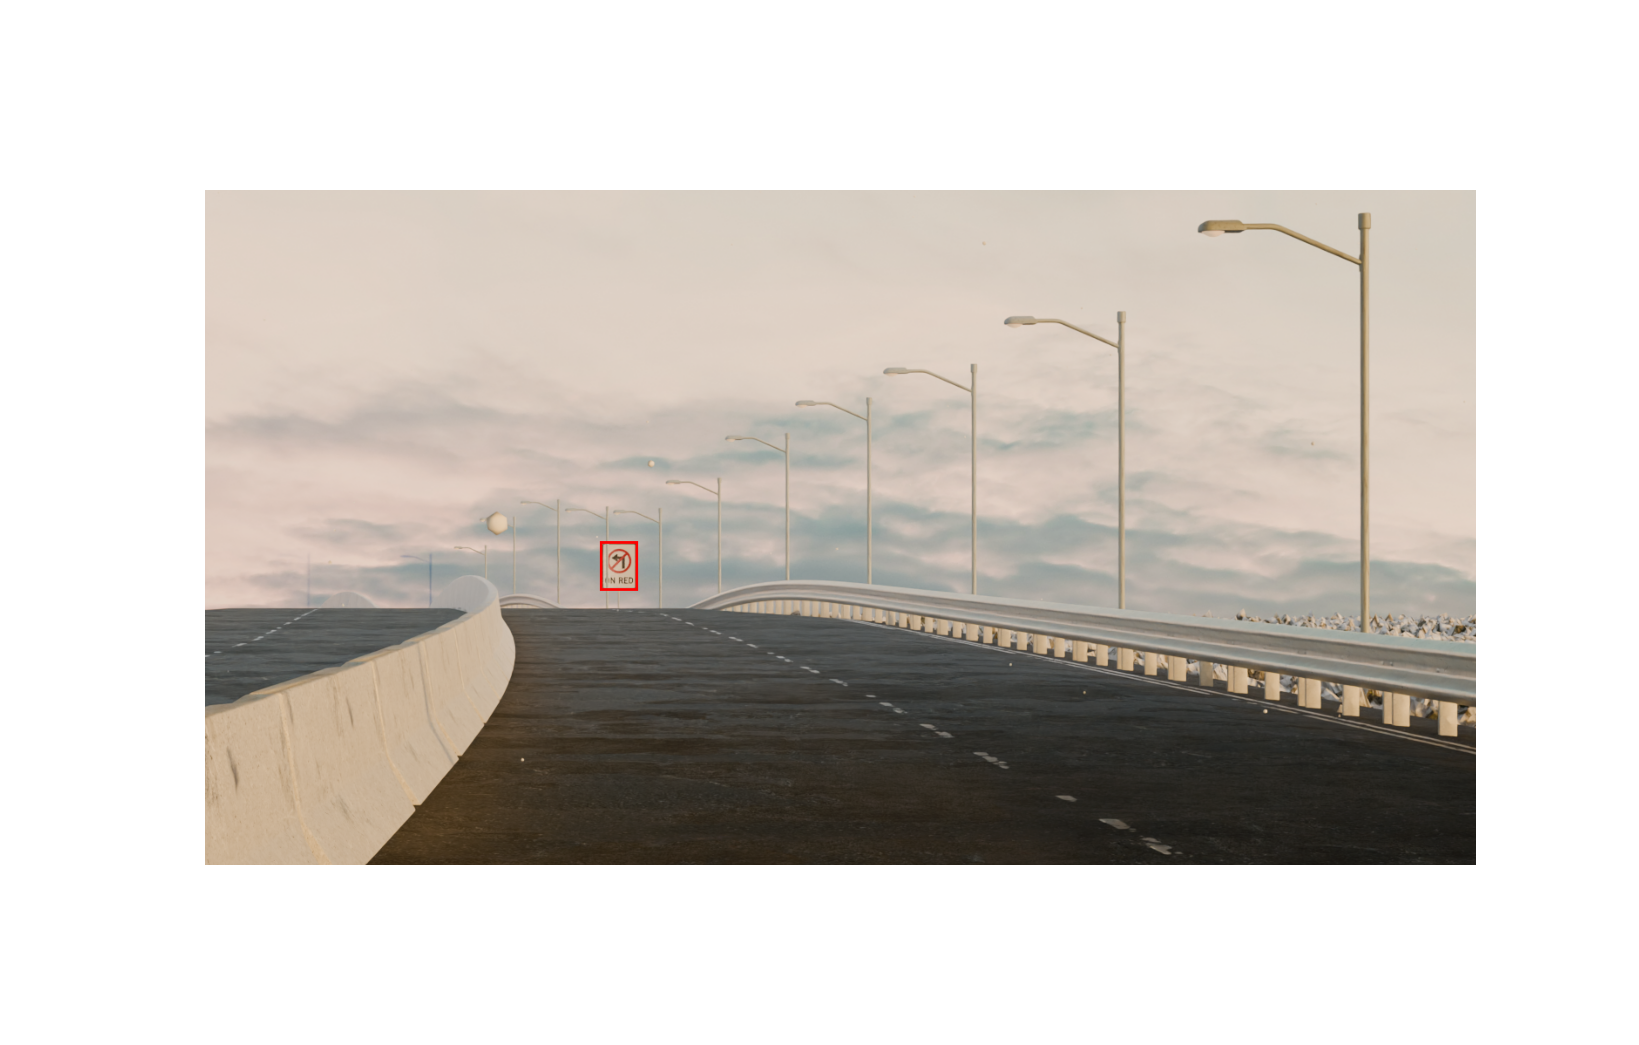
\includegraphics[width=\linewidth]{images/sign w box.png}
    \caption{Sample of generated image, including a red bounding box around the sign}
    \label{fig:row_of_images}
\end{figure}





\section{Results}
TO DO: Show generated images, train a model on a known dataset, train with just our dataset, and a combined dataset to show metrics

\section{Conclusion}
As signs are critical to safe and efficient roadways, it is important that detection models can quickly and correctly adapt to new road signs or locality-specific signs. Synthetic data, demonstrated here using a completely free blender pipeline, provides the means for quick and accurate tuning of existing training datasets. Although still somewhat limited by resources, the output dataset was successful in improving model performance with previously untrained signs. We are confident that this synthetic data generation tool will prove useful to sign detection models, as well as setting the groundwork for other road application such as sign size, road damage detection, and other environmental factors. 



% use section* for acknowledgment
\section*{Acknowledgment}


Sridhar, U of U Deep Learning Certificate program, state of Utah.... 


% Can use something like this to put references on a page
% by themselves when using endfloat and the captionsoff option.
\ifCLASSOPTIONcaptionsoff
  \newpage
\fi



% trigger a \newpage just before the given reference
% number - used to balance the columns on the last page
% adjust value as needed - may need to be readjusted if
% the document is modified later
%\IEEEtriggeratref{8}
% The "triggered" command can be changed if desired:
%\IEEEtriggercmd{\enlargethispage{-5in}}

% references section

% can use a bibliography generated by BibTeX as a .bbl file
% BibTeX documentation can be easily obtained at:
% http://mirror.ctan.org/biblio/bibtex/contrib/doc/
% The IEEEtran BibTeX style support page is at:
% http://www.michaelshell.org/tex/ieeetran/bibtex/
%\bibliographystyle{IEEEtran}
% argument is your BibTeX string definitions and bibliography database(s)
%\bibliography{IEEEabrv,../bib/paper}
%
% <OR> manually copy in the resultant .bbl file
% set second argument of \begin to the number of references
% (used to reserve space for the reference number labels box)
% \begin{thebibliography}{1}

% \bibitem{IEEEhowto:kopka}
% H.~Kopka and P.~W. Daly, \emph{A Guide to \LaTeX}, 3rd~ed.\hskip 1em plus
%   0.5em minus 0.4em\relax Harlow, England: Addison-Wesley, 1999.

% \end{thebibliography}
{\small
\bibliographystyle{unsrt}
\bibliography{bibtex/bib/bibliography}
}
% biography section
% 
% If you have an EPS/PDF photo (graphicx package needed) extra braces are
% needed around the contents of the optional argument to biography to prevent
% the LaTeX parser from getting confused when it sees the complicated
% \includegraphics command within an optional argument. (You could create
% your own custom macro containing the \includegraphics command to make things
% simpler here.)
%\begin{IEEEbiography}[{\includegraphics[width=1in,height=1.25in,clip,keepaspectratio]{mshell}}]{Michael Shell}
% or if you just want to reserve a space for a photo:

% \begin{IEEEbiography}{Michael Shell}
% Biography text here.
% \end{IEEEbiography}

% % if you will not have a photo at all:
% \begin{IEEEbiographynophoto}{John Doe}
% Biography text here.
% \end{IEEEbiographynophoto}

% % insert where needed to balance the two columns on the last page with
% % biographies
% %\newpage

% \begin{IEEEbiographynophoto}{Jane Doe}
% Biography text here.
% \end{IEEEbiographynophoto}

% You can push biographies down or up by placing
% a \vfill before or after them. The appropriate
% use of \vfill depends on what kind of text is
% on the last page and whether or not the columns
% are being equalized.

%\vfill

% Can be used to pull up biographies so that the bottom of the last one
% is flush with the other column.
%\enlargethispage{-5in}



% that's all folks
\end{document}


